\documentclass[12pt, a4paper]{article}
\usepackage[utf8]{inputenc}
\usepackage[english,russian]{babel}

\usepackage[centertags]{amsmath}
\usepackage{amsthm,amsfonts,amssymb}
\usepackage{indentfirst}

\frenchspacing
\parindent=0.6cm
\parskip=2pt
\mathsurround=1pt
%
\makeatletter
\renewcommand{\@biblabel}[1]{#1.}
\makeatother
%
\topskip=0mm
\headsep=0mm
\topmargin=0mm
\headheight=0mm
\textwidth=165mm
\textheight=240mm
\oddsidemargin=0mm

\renewcommand{\baselinestretch}{1.3}

%-------------------- END OF EXAMPLE ---------------------

\usepackage[mathscr]{euscript}
\usepackage{hyperref}
\usepackage{mathtext}
\usepackage[T2A]{fontenc}
\usepackage{graphicx}
\graphicspath{ {Images/} }
\usepackage[outdir=./Images/]{epstopdf}
\epstopdfsetup{update}
\usepackage{enumitem}
\usepackage{caption}
\usepackage{subfigure}
\usepackage{float}
\usepackage{amsthm}
\usepackage{amsmath}
\usepackage{soul}
%\usepackage{enumerate}
%\usepackage{vmargin}
%\usepackage[bottom,hang,stable]{footmisc}
%\usepackage{thmtools}

\theoremstyle{plain}
\newtheorem{theorem}{Теорема}
\newtheorem{lemma}{Лемма}
\newtheorem{corollary}{Следствие}
\newtheorem{proposition}{Предложение}
\newtheorem{assertion}{Утверждение}
\newtheorem*{assertion*}{Утверждение}

\theoremstyle{definition}
\newtheorem{definition}{Определение}
\newtheorem{remark}{Замечание}
\newtheorem{example}{Пример}


\theoremstyle{definition}
\newtheorem*{definition*}{Определение}

\newcommand{\explan}[1]{\Big\{\textit{ #1 } \Big\} }
\newcommand{\comb}[2]{\genfrac{(}{)}{0pt}{1}{#1}{#2}}
\renewcommand{\Pr}{\mathbb{P}}
\newcommand{\E}{\mathbb{E}}
\newcommand{\D}{\mathbb{D}}
\newcommand{\Sum}{\displaystyle\sum\limits}
\newcommand{\Max}{\max\limits}
\newcommand{\Min}{\min\limits}
\newcommand{\fromto}[3]{{#1}=\overline{{#2},\,{#3}}}
\newcommand{\floor}[1]{\left\lfloor{#1}\right\rfloor}
\newcommand{\ceil}[1]{\left\lceil{#1}\right\rceil}
\newcommand{\NN}{\mathbb{N}}
\newcommand{\RR}{\mathbb{R}}
\newcommand{\ZZ}{\mathbb{Z}}
\newcommand{\tild}{\widetilde}
\renewcommand{\le}{\leqslant}
\renewcommand{\ge}{\geqslant}
\renewcommand{\hat}{\widehat}
\renewcommand{\emptyset}{\varnothing}
\renewcommand{\epsilon}{\varepsilon}
\newcommand{\ol}{\overline}
\renewcommand{\phi}{\varphi}
\newcommand{\Alt}{\mathrm{Alt}\,}
\newcommand{\sm}{\text{ - }}
\renewcommand{\C}[2]{C_{#1}^{#2}}
\newcommand{\mc}[1]{\mathcal{#1}}
\newcommand{\quest}{\textbf{?????}}
\newcommand{\N}{\hat{N}}
\renewcommand{\D}{\widehat{D}}
\newcommand{\F}{\mathscr{F}}
\newcommand{\ceilfrac}[2]{\ceil{\frac{#1}{#2}}}
\renewcommand{\S}{\Sigma}
\newcommand{\hS}{\widehat{\S}}

% Switch off italics for new words
\renewcommand{\emph}[1]{\text{#1}}

\makeatletter
\def\@xfootnote[#1]{%
  \protected@xdef\@thefnmark{#1}%
  \@footnotemark\@footnotetext}
\makeatother
\begin{document}
\noindent УДК 519.1
\medskip

{\bfseries
С.\,А. Ложкин\footnote[1]{Факультет ВМК МГУ, проф., д.ф.-м.н.,
                       e-mail: lozhkin@cs.msu.su},
Л.\,И. Высоцкий\footnote[2]{Факультет ВМК МГУ, студ.,
                       e-mail: vysotskylev@yandex.ru}
\medskip

О НЕКОТОРЫХ АСИМПТОТИЧЕСКИ ОПТИМАЛЬНЫХ \\
\indent ОДНОСТОРОННИХ ВЛОЖЕНИЯХ  ДЕРЕВЬЕВ ПОДОБНЫХ \\
\indent ФОРМУЛ  В ПРЯМОУГОЛЬНЫЕ РЕШЕТКИ
}

\begin{quotation}{\footnotesize
В данной работе рассматривается задача оптимального размещения в прямоугольных 
решетках деревьев формул. Проведено построение 
и анализ двух типов указанных деревьев и соответствующих способов их вложения (размещения) в 
такие решетки: 
на основе полных двоичных деревьев и на основе специальных двоичных деревьев.
Для вложений деревьев второго типа доказана асимптотическая оптимальность по высоте получаемой решетки 
среди деревьев всех подобных исходной формуле формул не большей глубины.
  \\
 \indent\textit{Ключевые слова}: вложение деревьев, прямоугольные
  решетки, подобные формулы, оптимизация по высоте.}
\end{quotation}
\medskip

{\bfseries 1. Введение.}\ 
Проблема оптимального взаимного моделирования вычислений является 
одной из актуальных задач теории дискретных управляющих систем.
Обычно она сводится к задаче оптимизации размещения
вычислительных узлов и связей между ними в геометрических структурах определенного вида, например, в прямоугольной решетке.

В такой постановке проблема возникает при проектировании различных
цифровых и аналоговых схем в связи со стремлением производителей минимизировать размеры своего продукта, к примеру, при разработке сверхбольших интегральных схем или блока  дискретного преобразования Фурье --- важной части цифрового сигнального процессора.

В качестве модели геометрической структуры были выбраны прямоугольные решетки, в узлах которых можно
размещать вычислительные узлы, а по ребрам проводить соединяющие их проводники. 
Моделью размещаемого устройства являются деревья формул над произвольным базисом
двуместных ассоциативных и коммутативных операций. 
Само размещение задается т.\,н. вложением, т.\,е. отображением вершин дерева в узлы, а ребер ---
в непрерывные цепи решетки. На это отображение могут накладываться определенные ограничения,
следующие из физических или технологических особенностей моделируемой системы.
Например, в данной работе требуется, чтобы цепи--образы ребер не пересекались друг с другом
в узлах, отличных от вычислительных, а входы устройства располагались на одной 
(горизонтальной) стороне решетки.

Рассматривается следующая задача: для заданной формулы 
среди всех подобных ей (т.е. получающихся из нее применением тождеств
ассоциативности и коммутативности) формул определенной глубины найти такую,
для которой возможно указанное выше вложение в решетку минимальной высоты. 
%Подобными
%называются формулы над базисом ассоциативных и коммутативных операций,
%если одну можно получить из другой, применяя тождества ассциативности
%и коммутативности. 

В данной работе приводится метод построения искомых подобных формул 
и их вложений на основе полных двоичных деревьев, а также
на основе специальных двоичных деревьев.
Для последнего метода доказана его асимптотическая оптимальность
в смысле описанной задачи.
\smallskip

{\bfseries 2.
Постановка задачи и формулировка полученных результатов.
}
%
%
%\subsubsection{Формулы}
Приведем определение формулы (те понятия, которые здесь не определены, могут быть найдены в \cite{cyber}). Пусть задан счетный упорядоченный \emph{алфавит переменных} 
$\mathscr{X} = \{ x_1, x_2, \dots, x_n, \dots \}$, а также базис $Б = \{\phi_1, \phi_2, \dots, \phi_b\}$,
где $\phi_i$ --- $k_i$-местная функция. Формула над  базисом Б задается рекуррентно:
 переменная $x_j \in \mathscr{X}$ считается формулой;  если $\F_1, \dots, \F_{k_i}$ --- формулы, то запись вида
$\F = \phi_i(\F_1, \dots, \F_{k_i})$ тоже
считается формулой. В данной работе рассматривается
базис двуместных ассоциативных и коммутативных функций.
Каждой формуле естественным образом ставится в соответствие реализуемая ею функция, а также
дерево, листья которого помечены переменными, а нелистовые вершины --- функциями из базиса Б.
\emph{Сложностью} $L(\F)$ формулы $\F$ называется число вхождений в нее функциональных символов, ее \emph{глубиной} --- глубина соответствующего дерева, а \emph{альтернированием} $\Alt(\F)$ --- максимальное число изменений пометок функций вдоль 
пути от листа дерева, соответствующего формуле $\F$, до его корня. Формула $\F_2$ называется \emph{подобной} формуле $\F_1$, если $\F_2$ может быть получена из $\F_1$ путем нескольких 
эквивалентных преобразований с помощью тождеств ассоциативности и коммутативности для базисных функций.

Рассматриваются неориентированные графы без петель и кратных ребер. Они представляют собой пару множеств
$G = (V_G, E_G)$, где $V_G$ и $E_G$ --- множества вершин и ребер соответственно. Множество всех простых (без самопересечений) цепей графа $F$ будем обозначать $C(F)$.

\emph{Вложением} графа $G$ в граф $F$ назовем пару отображений $(\phi, \psi)$:
\[
	\phi~:~V_G \rightarrow V_F, ~~ \psi~:~E_G \rightarrow С(F),
\]
обладающую тем свойством, что для любого ребра $e = (u, v) \in E_G$ цепь $\psi(e)$
соединяет вершины $\phi(u)$ и $\phi(v)$. При этом
образы вершин из $V_G$ будем называть \emph{основными} вершинами вложения,
цепи, являющиеся образами ребер из $E_G$, --- \emph{транзитными} цепями вложения,
ребра и внутренние вершины (т.\,е. не совпадающие с концами) транзитных цепей --- \emph{транзитными} ребрами и вершинами соответственно.


Будем рассматривать лишь те вложения, для которых различные вершины графа $G$ переходят в различные
вершины графа $F$, транзитные цепи не имеют общих ребер, а через одну транзитную вершину
проходит не более 1 транзитной цепи.

Обозначим через $A^{a,b}_{l, h}$ целочисленную прямоугольную решетку (ПР) высоты $h$ и длины $l$ с началом в точке
$(a,b)$, т.\,е. граф, множеством вершин которого является множество точек $(x, y)$ плоскости с целочисленными 
координатами из прямоугольника 
$
	[a, a + (l - 1)] \times [b, b + (h - 1)],
$
а ребра соединяют все пары точек $(x_1, y_1)$ и $(x_2, y_2)$, таких, что 
$|x_1 - x_2| + |y_1 - y_2| = 1$. Если не оговорено иное, будем считать, что $a=b=0$, а $h \le l$.
	
Вложение дерева в ПР назовем \emph{каноническим}, если образ корня находится
в первой строке решетки (т.\,е. имеет ординату 0), и \emph{строго каноническим}, если дополнительно
он является единственной основной вершиной в первой строке решетки.

 Рассматривается следующая задача: для формулы $\F$ над конечным базисом  (хотя результат естественным образом обобщается и на бесконечный базис)
$Б$ из коммутативных и ассоциативных функций  построить подобную ей формулу $\F'$ минимальной
глубины, допускающую вложение ее дерева в ПР минимальной высоты с расположением листьев на одной стороне решетки. При этом в ситуации
неоднозначности решения задачи минимизации двух функционалов была выбрана
следующая интерпретация: необходимо построить формулу $\F'$ глубины не более 
$
\log L(\F) + c\, \Alt (\F) + 1
$ 
(все логарифмы, если не указано иное, берутся по основанию 2),
где $c$ --- некоторая константа, и с минимальной высотой решетки, в которую возможно ее вложение.

В данной работе приведен метод построения для произвольной 
формулы $\F$ в базисе двуместных коммутативных и ассоциативных
операций подобной ей формулы $\F_1$ глубины
не более $d_1 = \ceil{\log (L(\F) + 1)} + \Alt(\F)$
с указанием канонического вложения дерева формулы $\F_1$ в прямоугольную решетку высоты не более
$
	\floor{d_1 / 2} + 1.
$
Также разработан метод построения подобной формуле $\F$ формулы $\F_2$ глубины 
не более 
\[
	d_2 = \ceil{\log (L(\F) + 1) + \log  6 \cdot \Alt(\F)} + 1,
\]
с указанием канонического вложения дерева формулы $\F_2$ в прямоугольную решетку высоты не более
$
	(d_2/3)(1 + o(d_2)),
$
которое является асимптотически оптимальным среди всех вложений деревьев рассматриваемых формул глубины не более $d_2$.
%
%В определенном смысле $\log L(\F) + \Alt(\F)$ есть минимальная (в худшем случае) глубина формул, подобных $\F$. 
%Формально говоря, несложно построить последовательность формул $\{\F_n\}$ со свойством
%$L(\F_n) = \Alt(\F_n) - 1 = n$, для которой 
%$\Min_{\F'_n \text{ подобна } \F_n} D(\F'_n) = L(\F_n)$, что асимптотически равно $\log L(\F_n) + \Alt(\F_n)$.
%С другой стороны, в каком-то смысле произвольный постоянный множитель при $\Alt(\F)$ 
%в выражении 
%$
%\log L(\F) + c \cdot \Alt (\F) + 1
%$
%свидетельствует о том, что
%постановка задачи ориентирована  на класс формул, в которых $\Alt(\F) = const$ или $\Alt(\F) \ll \log L(\F)$,
%благо многие важные классы (к примеру, ДНФ, КНФ и полиномы Жегалкина) обладают этим свойством.


\bigskip

{\bfseries 3. Вложение деревьев формул на основе полных двоичных деревьев.}

Для построения эффективных вложений в дальнейшем будем
использовать идею композиции вложений. Формально, если 
заданы два вложения $(\phi_1, \psi_1)$ и $(\phi_2, \psi_2)$:
\[
	G \xrightarrow{~\phi_1, \psi_1~} F \xrightarrow{~\phi_2, \psi_2~} H,
\]
то можно естественным образом определить новое вложение $(\phi, \psi)$:
\[
\phi(v) = \phi_2(\phi_1(v)), ~~~ \psi(e) = \psi_2(e'_1) \Cup \dots\Cup\psi_2(e'_n),
\]
где $(e'_1, \dots, e'_n) = \phi_1(e)$, а $\Cup$ -- операция конкатенации цепей. 
Заметим, что построенная пара функций действительно будет вложением: все цепи $\psi(e)$ будут простыми, так как две различные цепи $\psi_2(e')$ и $\psi_2(e'')$ могут пересечься
лишь в основных вершинах вложения $(\phi_2, \psi_2)$.

В наших дальнейших рассуждениях будут строиться композиции
вида $F \rightarrow D \rightarrow A$, где $F$ -- некоторое дерево формулы, $D$ -- дерево с некоторой регулярной структурой (например, полное), а $A$ -- прямоугольная решетка.

Заметим, что вложение одного дерева в другое обладает тем свойством, что оно полностью определяется отображением вершин. Действительно, в дереве существует ровно один путь между любыми двумя вершинами, позволяя определить $\psi(e)$ однозначно.

%\begin{mylemma} \label{vertexdepth} Существует строго каноническое вложение полного двоичного дерева глубины $d$ 
%в решетку высоты $\ceil{d/2} + 1$, причем такое, что образ любой вершины на глубине (т.е. расстоянии от корня) $\hat{d}$ имеет 
%ординату $\ceil{\widehat{d} / 2}$.
%\end{mylemma}
%\begin{myproof} При четной глубине первая часть утверждения леммы следует из леммы 4 статьи \cite{lidamin}.
%При нечетной глубине для дерева высоты 1 нужно взять вложение, изображенное на Рис. \ref{img1:base2},
%а дальнейшее построение проводить аналогично (Рис. \ref{img1:buildnotgrow}
%и \ref{img1:buildgrow}).
%
%Осталось доказать вторую часть леммы. Ясно, что ордината образа $(x, y)$ вершины $v$ равна разности $H - h$,
%где $H$ --- высота вложения всего дерева $D$, а $h$ --- высота вложения поддерева с корнем в $v$. По построению
%рассуждение разбивается на два случая: для четного и нечетного $d$. Рассмотрение обоих случаев требует тривиальных выкладок
%с использованием свойств функций $\ceil{\cdot}$ и $\floor{\cdot}$.
%\end{myproof}

\begin{figure*}[h]
\begin{minipage}[h]{0.24\linewidth}
\center{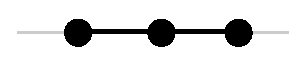
\includegraphics[width=0.75\linewidth]{base_1} \\ \textit{а}}
\end{minipage}
\hfill
\begin{minipage}[h]{0.24\linewidth}
\center{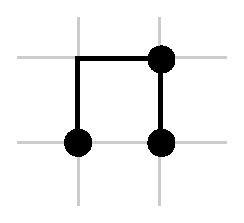
\includegraphics[width=0.5\linewidth]{base} \\ \textit{б}}
\end{minipage}
\begin{minipage}[h]{0.24\linewidth}
\center{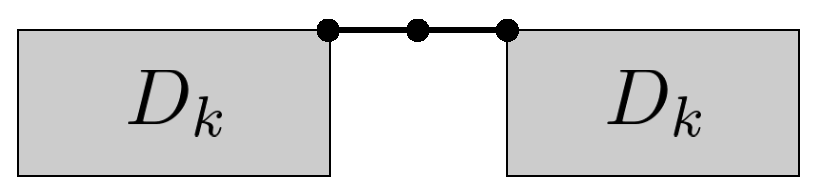
\includegraphics[width=0.9\linewidth]{building_not_grow} \\ \textit{в}}
\end{minipage}
\hfill
\begin{minipage}[h]{0.24\linewidth}
\center{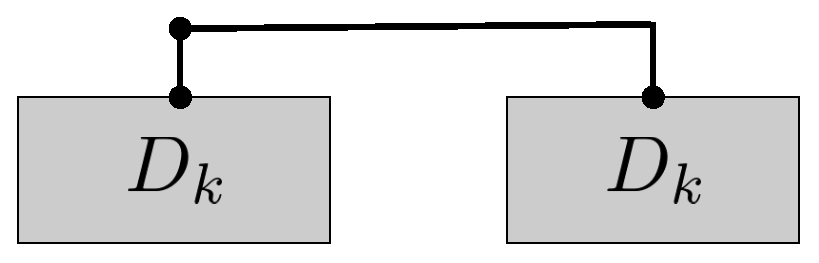
\includegraphics[width=0.9\linewidth]{building_grow} \\ \textit{г}}
\end{minipage}

\captionsetup{labelformat=empty}{Построение канонических вложений полного двоичного дерева: \textit{а} --- базовое каноническое вложение дерева $D_1$; \textit{б} --- базовое строго каноническое вложение $D_1$; \textit{в} ---
каноническое вложение дерева $D_{k+1}$(для строго канонического
вложения $D_k$); \textit{г} --- строго каноническое вложение дерева $D_{k+1}$ 
 (для нестрого канонического
 вложения $D_k$)}
\label{ris:image1}
\end{figure*}


%\begin{mylemma} \label{compositionmapping} 
%Пусть заданы два двоичных дерева $D_1$  и $D_2$, причем в дереве $D_1$ выделен лист $v$. Пусть также заданы 
%вложения деревьев $D_1$  и $D_2$ в решетки высоты $h_1$ и $h_2$ соответственно, причем образ листа $v$ имеет координаты $(x_v,y_v)$, вершины $(x_v,y_v+1), (x_v,y_v+2), \dots ,(x_v,h_1-1)$ являются свободными, а вложение дерева $D_2$ является строго каноническим.
%
%Тогда существует вложение дерева $D$, полученного 
%отождествлением корня дерева $D_2$ с листом $v$, в решетку высоты не более $y_v + h_2$.
%\end{mylemma}
%\begin{myproof}
%Дополним решетку вложения $D_1$ свободными строками до высоты $y_v + h_2$ (если
%$y + h_2 \le h_1$, то делать ничего не надо).
%
%Введем операцию \emph{расширения на длину $\ell$} решетки растяжением
%ребер между столбцами с абсциссами $x$ и $x + 1$ следующим образом:
%заменим каждое ребро $(x,y)\text{ - }(x+1,y)$ цепью 
%$(x,y)\text{ - }(x+1,y)\text{ - }(x+2,y)\text{ - }\dots\text{ - }(x+\ell + 1,y)$,
%соответствующим образом увеличив все абсциссы вершин правее модифицируемых столбцов,
%а также добавив соответствующие вертикальные ребра (между добавленными вершинами).
%При этом в случае, если ребро $(x,y)\text{ - }(x+1,y)$ было свободным,
%добавляемую цепь объявим свободной, а если оно было транзитным, объявим
%цепь транзитной.
%Данная операция наглядно изображена на Рис. \ref{img2}.
%Ясно, что в результате получается вложение того же графа. 
%
%
%Рассмотрим теперь вложение дерева $D_2$. Пусть оно имеет ширину $w_2$.
%Вследствие каноничности вложения образ расположен в верхней строке решетки,
%а вследствие строгой каноничности его (образ) можно перенести влево или вправо вдоль транзитных ребер
%таким образом, что слева (соответственно справа) от него будет свободное ребро. 
%Направление переноса выберем в зависимости от того, с какой стороны к образу листа $v$
%примыкает транзитное ребро: если слева, то переносить образ корня $D_2$ будем также влево;
%если справа, то переносить будем вправо; а если сверху, то без разницы. Заметим, что в силу условия 
%леммы ребро, инцидентное снизу, является свободным.
%
%Обозначим новые координаты образа корня дерева $D_2$ за 
%за $(x_2, y_2)$. Применим к решетке вложения $D_1$ операцию расширения на длину $w_2 - x_2$ к столбцам с абсциссами $x_v$  и $x_v+1$,
%а затем операцию расширения на длину $x_2$ к столбцам с абсциссами $x_v - 1$ и $x_v$.
%В результате этих операций образ $v$ переместился в $(x_v', y_v)$, где $x_v' = x_v + x_2$ (а ордината не могла измениться
%в результате этих операций).
%
%Рассмотрим подрешетку 
%$
%L = [x_v'-x_2, x_v' + w_2 - x_2 - 1] \times [y_v, y_v + h_2 - 1]
%$
%(под $[a,b]$, где $a,b\in \ZZ$, если не указано иное, имеется в виду множество $\{k\in\ZZ:~a \le k \le b\}$).
%
%До операции расширения ребра $(x_v, y)\text{ - }(x_v + 1, y)$, $(x_v, y-1)\text{ - }(x_v, y)$
%и $(x_v - 1,y)\text{ - }(x_v, y)$ для $y \in [y_v + 1, h_1 - 1]$, были свободными (иначе одна из вершин
%$(x_v, y)$ оказалась бы транзитной или основной).
%Значит, по определению операции расширения, все ребра и вершины подрешетки $L$ являются свободными,
%за исключением, возможно, ребер и вершин первой строки. Для первой строки либо 
%ребра справа от $(x_v',y_v)$ являются свободными, либо ребра слева.
%
%Теперь можем наложить решетку вложения $D_2$ на $L$, так как они имеют одинаковые размеры. При этом транзитные ребра наложатся только на свободные
%ребра, транзитные и основные вершины -- на свободные вершины, за исключением образа корня $D_2$ -- 
%он будет совмещен с образом $v$, что и требовалось.
%\end{myproof}
% 
% \begin{figure}[ht]
%
% \subfigure[Вложение до операции расширения. Черным цветом отмечены транзитные ребра и основные вершины вложения,
%  серым -- свободные ребра]{%
% \includegraphics[width=0.40\textwidth]{Images/before_cut_expand.pdf}
% \label{img2:before}}
% \subfigure[Вложение после операции расширения. Новые вершины помечены серыми квадратиками]{
% \includegraphics[width=0.45\textwidth]{Images/after_cut_expand.pdf}
% \label{img2:after}}
% 
% \caption{Иллюстрация операции расширения на 1}
% \label{img2}
% \end{figure}
\begin{theorem}
	\label{thm:full}
 Для любой формулы $\F$ в базисе двуместных коммутативных и ассоциативных
функций $Б = \{\phi_1, \dots, \phi_b \}$ существует подобная ей формула $\F'$ глубины
не более $d = \ceil{\log (L(\F) + 1)} + \Alt(\F),$
а также каноническое вложение дерева этой формулы в прямоугольную решетку высоты не более
$
	\floor{d / 2} + 1.	
$
\end{theorem}
\begin{proof} 
Построим искомое вложение как композицию двух вложений.
Сначала найдем  подобную $\F$ формулу $\F'$, дерево которой мы могли бы вложить в
полное двоичное дерево $D$ глубины $d$,
а затем воспользуемся доказанным в \cite{lidamin} фактом о вложении полного дерева в ПР высоты $\floor{d/2}+1$ (см. рисунок).

Покажем индукцией по сложности, что для $\F$ существует подобная формула $\F'$ и ее вложение в полное 
двоичное дерево глубины $\ceil{\log (L(\F) + 1)} + \Alt(\F)$.

База ($L(\F) = 1$) очевидна: $\F' = \F = x_i$.
Обоснуем шаг индукции.
Представим формулу $\F$ в виде
$
	\F = \F_1 \circ \F_2 \circ \dots \circ \F_s,
$
где $\circ \in Б$. По аналогии c теоремой 2.1 из \cite{cyber} выделим	 в полном дереве глубины $d$ непересекающиеся поддеревья $D_i$, $i=1,\dots,s$, глубины $d_i = \ceil{\log (L(\F_i) + 1)} + \Alt(\F_i)$ и обозначим через $v_i$ корень дерева $D_i$. Применим индуктивное предположение к
подформулам $\F_i$, $i=1,\dots,s$, построив подобные им формулы $\F_i'$
и их вложения в $D_i$. Рассмотрим такой подграф $T$ дерева $D$, который сам явяется деревом, имеет корень в корне $D$, а листьями являются только вершины $v_i$, $i=1,\dots,s$. 
Это можно сделать, рассмотрев в качестве такого подграфа объединение всех цепей, соединяющих $v_i$, $i=1,\dots,s$, с корнем $D$.

Построим формулу $\mathscr{H}(y_1, \dots, y_s)$ следующим образом:
рассмотрим в дереве $T$ множество $W \subset V_T$, состоящее из всех вершин степени 3 (и корня, если его степень равна 2) и листьев, а затем 
проведем ребро $(w_1, w_2)$, если путь от $w_1$ до $w_2$ (определяемый однозначно)
не содержит других вершин из $W$.
Ясно, что полученный граф $T' = (W, E_{T'})$ является деревом:
связность и наличие ровно одного пути между вершинами из $W$ следует из построения. Корнем $T'$ назначим ближайшую к корню дерева $D$ вершину.
Это и будет дерево формулы $\mathscr{H}$ --- достаточно приписать всем вершинам функциональный символ
$\circ$. Вложение $T' \rightarrow T$ очевидно из построения. 


Теперь определим формулу $\F' = \mathscr{H}(\F'_1, \dots, \F'_s)$. 
Ее вложение в дерево $D$ определяется однозначно на основе вложений
$\F'_i \rightarrow D_i$, а также $\mathscr{H} \rightarrow T$. 
Несложно также видеть, что глубина формулы $\F'$
не превосходит глубины $D$.
Теорема доказана.
\end{proof}
\bigskip

{\bfseries 4. Вложение деревьев формул на основе специальных двоичных деревьев.} \
В работе \cite{lidamindis} описываются двоичные деревья,
имеющие максимальное число листьев среди деревьев глубины не
более $d$ и допускающие вложение в решетку высоты не более
$h$. Это максимальное число листьев, зависящее от $d$ и $h$, обозначается через $N(d,h)$ и равно 
\[
	N(d, h) = 2^d - 2^h \sum_{k = 0}^{d - 2h} \C{d-h}{k}.
\]
Оказывается, при построении различных схем, оптимальных по высоте или площади вложения в прямоугольные решетки, во многих случаях
разумнее использовать указанные ``специальные'' деревья вместо ``классических''  полных.
\smallskip

{\bfseries 4.1. Асимптотически оптимальное по высоте вложение  деревьев формул.} \ 
Рассмотрим деревья $\hat{D}(d,h)$ (определяемые лишь при $d \le 3h+2$)
и $\hat{D}_L(d,h)$ (определяемые лишь при $d \le 3h+1$),
которые в случае $d = 0$ представляют собой отдельные вершины, а при $d > 0$ задаются рекуррентно следующим образом:
\begin{enumerate}[label={\arabic*)}]
\item $\hat{D}(d,h)$ имеет два одинаковых поддерева $\hat{D}_L(d-1,h)$;
\item $\hat{D}_L(d,h)$ при $d = 3h + 1$ имеет два поддерева
$\hat{D}_L(d-2,h)$ и $\hat{D}(d-2,h-1)$,
а при $d \le 3h$ два поддерева $\hat{D}_L(d-1,h)$ и $\hat{D}(d-1,h-1)$
(таким образом, деревья $\hat{D}_L(3h + 1, h)$ и $\hat{D}_L(3h, h)$ совпадают).
\end{enumerate}
Заметим, что глубина деревьев $\hat{D}(d,h)$ и $\hat{D}_L(d,h)$ 
не превосходит $d$. Кроме того, для них 
 несложно определить каноническое 
 вложение в решетку высоты $h$. Дерево $\hat{D}(d,h)$ назовем регулярным симметричным, а $\hat{D}_L(d,h)$ --- регулярным асимметричным.
Для числа листьев у рассматриваемых деревьев можно
записать следующие рекуррентные соотношения:
\begin{equation}
\label{eq:recur1}
\hat{N}(d,h) = 2\hat{N}_L(d-1,h),
\end{equation}
\begin{equation}
\label{eq:recur2}
\hat{N}_L(d,h) = 
\begin{cases}
	2\hat{N}(d-1,h-1) + \hat{N}_L(d-1,h),&~\text{если}~d \le 3h,\\
	\hat{N}_L(d-1,h),&~\text{иначе.}
\end{cases}
\end{equation}
По построению первое соотношение должно выполнятся при всех $d \le 3h + 2$,
а второе --- при всех $d \le 3h + 1$.

\smallskip

{\bfseries 4.2. Вспомогательные утверждения.} \
\begin{lemma}
Пара функций 
\begin{equation}
\label{eq:hatN}
\hat{N}(d,h) =2^h\Sum_{k=d-2h+1}^{h+3}C_{d-h}^k
,~~~\hat{N}_L(d,h) = \frac{1}{2}\hat{N}(d+1,h)
\end{equation}
удовлетворяет соотношениям \textnormal{(\ref{eq:recur1})}\textup{,} \textnormal{(\ref{eq:recur2})}.
\end{lemma} 

\begin{proof}
Соотношение (\ref{eq:recur1}), очевидно, выполнено. 
Перепишем соотношение (\ref{eq:recur2}), выразив $\hat{N}_L(d,h)$ через $\hat{N}(d,h)$:
\[
\hat{N}(d+1,h) = 
\begin{cases}
	2\hat{N}(d-1,h-1) + \hat{N}(d,h),&~\text{если}~d \le 3h,\\
	\hat{N}(d,h),&~\text{иначе.}
\end{cases}
\]

В обоих случаях равенство проверяется прямой подстановкой и 
применением тождества $C_{n}^k = C_{n-1}^k + C_{n-1}^{k-1}$.
Лемма доказана.
\end{proof}

\begin{lemma}[о регулярном делении]
\label{lemma:reg}
Для величины $r(d,h)$\textup{,} определяемой равенством
\[
r(d,h) = \frac{\hat{N}_L(d-1,h)}{\hat{N}_L(d,h)},
\]
при $h > 1$ и $d \le 3h$ выполнены неравенства
$
	1/2 \le r(d,h)  \le 5/6.
$
\end{lemma}

\begin{proof}
В соответствии с доказанным рекуррентным соотношением (\ref{eq:hatN})
\[
r(d,h) = \frac{\hat{N}(d,h)}{\hat{N}(d+1,h)} = \frac{\Sum_{k=d-2h+1}^{h+3}C_{d-h}^k}{\Sum_{k=d-2h+2}^{h+3}C_{d-h + 1}^k} = \frac{\Sum_{k=d-2h+1}^{h+3}C_{d-h}^k}{2\Sum_{k=d-2h+1}^{h+3}C_{d-h}^k - C_{d-h}^{d-2h+1} - C_{d-h}^{h+3}}.
\]
%
Отсюда сразу видно, что $r(d,h) \ge 1/2$, так как знаменатель не превосходит удвоенный числитель. 
Для получения верхней оценки величины $r(d,h)$ достаточно оценить величины
\[
	A(d,h) = \frac{ C_{d-h}^{d-2h+1} + C_{d-h}^{h+3} }{\Sum_{k=d-2h+1}^{h+3}C_{d-h}^k} = \frac{ C_{d-h}^{d-2h+1} + C_{d-h}^{h+3} }{C_{d-h}^{d-2h+1} + \Sum_{k=d-2h+2}^{h+2}C_{d-h}^k + C_{d-h}^{h+3}} = 
	\frac{1}{1 + B(d,h)},
\]
\[
B(d,h) = \frac{\Sum_{k=d-2h+2}^{h+2}C_{d-h}^k }{C_{d-h}^{d-2h+1} + C_{d-h}^{h+3}}.
\]
Для установления нижней оценки величины $B(d,h)$ заметим, что в условиях леммы (т.\,е. при $d \le 3h$)
верно неравенство $h+2>(d-h)/2$, из которого вытекает неравенство $C_{d-h}^{h+2} > C_{d-h}^{h+3}$.  Заметим также , что при $d < 3h-2$ выполняется неравенство $d-2h+1 < (d-h)/2$, из чего следует, что $ C_{d-h}^{d-2h+1} \le C_{d-h}^{d-2h+2}$. 
Учитывая это, достаточно рассмотреть случаи $d < 3h - 2$, $d= 3h-2$, $d= 3h-1$ и $d= 3h$. В результате для любых $d$ и $h$ из условия леммы получим оценку $B(d,h) \ge 1/4$. Значит,
\[
	r(d,h) = (2 - A(d,h))^{-1} = (2 - \frac{1}{1 + B(d,h)})^{-1} \le \frac{5}{6}. 
\]
Лемма доказана.
\end{proof}
 

Для удобства формулирования следующей леммы доопределим $\N_L(d,h)$ 
в точке $(3h+2,h)$: $\N_L(3h+2,h) = \N_L(3h+1,h)$. 
 
\begin{lemma}
\label{lm:key}
Пусть заданы натуральные числа $m_1, \dots, m_n,$ сумма которых равна $M$. 
Тогда для целых неотрицательных чисел $d$ и $h$\textup{,} таких\textup{,} что $d \le 3h + 2$ и $\N(d,h) \ge M$ \textup{(}соответственно $d \le 3h + 1$ и $\N_L(d,h) \ge M$\textup{)} 
в дереве $\hat{D}(d,h)$ \textup{(}соответственно $\hat{D}_L(d,h))$ можно выделить $n$ попарно не пересекающихся поддеревьев $D_1, \dots, D_n$\textup{,} таких\textup{,} что 
число $N_i$ листьев дерева $D_i$, $i=1,\dots,n,$
удовлетворяет следующим неравенствам\textup{:}
\begin{equation}
\label{eq:conditions}
N_i \ge \begin{cases} 
										m_i,&~~\text{если}~n=1,\\
									   \frac{1}{6} m_i,& ~~\text{если}~n>1 ~~\text{и}~~1 < i < n,\\
                                       \frac{1}{3}   m_i,& ~~\text{если}~n>1 ~~\text{и}~~i \in \{1,n\}.
                         \end{cases}
\end{equation}
\end{lemma} 


\begin{proof}
Проведем индукцию по $n=1,2,\dots$.
Для $n=1$ лемма очевидно верна.

Докажем сначала часть утверждения, связанную с деревом $\hat{D}_L(d,h)$, причем рассмотрим случай $d \le 3h$ (случай $d = 3h+1$ тривиален, так как $\hat{D}_L(3h+1,h) = \hat{D}_L(3h,h)$). Положим $r = r(d,h)$ (см. лемму \ref{lemma:reg}) и будем считать, что $ M r$ --- целое число.
Если это не так, то положим $M' = r\ceil{M/r}$ и соответствующим 
образом увеличим любое из чисел $m_i$.
Ясно, что так как $\N_L(d,h) r = \N_L(d-1,h)$ --- целое число и $\N_L(d,h) \ge M$, то 
$M' \le \N_L(d,h)$, т.\,е. условия леммы выполняются, а  результирующие соотношения (\ref{eq:conditions}) 
лишь усилятся.

Выберем номера $k_1$ и $k_2$, такие, что 
\begin{equation*}
\begin{split}
	\Sum_{i=1}^{k_1}m_i \ge (1- r)  M,& ~~~~ \Sum_{i=1}^{k_1-1} m_i < (1-r)  M,\\	
	\Sum_{i=1}^{k_2}m_i \ge r M,& ~~~~ \Sum_{i=1}^{k_2-1} m_i < r M.\\
\end{split}
\end{equation*}

При этом возможны две ситуации.

1. $\{k_1,k_2\} \subseteq \{1,n\}$. Рассмотрим два случая:

$\mspace{20mu}$а) $k_1 = k_2$. В этом случае без ограничения общности будем
 считать, что $k_1 = k_2 = 1$. Применим индуктивное предположение к поддереву $\hat{D}_L(d-1,h)$ с набором
$\mathcal{M}_1 = \{rM\}$ и к поддереву
$\hat{D}(d-1,h-1)$ c набором $\mathcal{M}_2 = \{m_2, \dots,m_n\}$. В силу того, что $m_1 \le M$ и $r \ge 1/2$,
получим выполнение всех условий (\ref{eq:conditions}) 
для системы поддеревьев $S$ дерева $\hat{N}_L(d,h)$ с набором
$\mathcal{M} = \{m_1, \dots, m_n\}$, которая является 
объединением указанных подсистем.

$\mspace{20mu}$б) $k_1 \neq k_2$. Так как $k_1 \le k_2$, то $k_1 = 1,~k_2 = n$. Без ограничения общности можно 
считать, что $m_1 \le m_n$.
Применим индуктивное предположение к поддереву $\hat{D}(d-1,h-1)$ с набором
$\mathcal{M}_1 = \{(1-r) M\}$ (ведь $(1-r)M = \hat{N}(d-1,h-1)$) и к поддереву
$\hat{D}_L(d-1,h)$ c набором $\mathcal{M}_2 = \{m_2, \dots,m_n\}$. Выполнение условия (\ref{eq:conditions}) 
для определенной аналогично системе $S$ системы нужно проверить лишь для $N_1$. Учитывая, что $m_1 \le m_n$, а значит,  $M \ge 2m_1$, и применяя лемму \ref{lemma:reg}, получим
\[
N_1 \ge (1-r)  M \ge (1-r)2m_1 \ge \frac{2}{6} m_1 = \frac{1}{3}m_1.
\]


2. $\{k_1,k_2\} \not \subseteq \{1,n\}$. Пусть для определенности $k_1 \notin \{1,n\}$. Введем обозначения
\[
M^L = (1-r)M,~~~ M^R = r M,~~~ m_k^L = M^L - \Sum_{i=1}^{k-1}m_i,~~~m_k^R = \Sum_{i=1}^{k}m_i - M^L
\] 
и, не ограничивая общности рассуждений, будем считать, что $m_k^L \ge m_k^R$. Применим индуктивное предположение к поддереву $\hat{D}(d-1,h-1)$ с набором $\{m_1, \dots, m_k^L\}$ и поддереву $\hat{D}_L(d-1,h)$ с набором $\{m_{k+1}, \dots, m_n\}$.
Среди условий (\ref{eq:conditions}) для определенной аналогично системе $S$ системы нужно проверить лишь условие для $N_k$:
\[
	N_k \ge \frac{1}{3} m_k^L \ge \frac{1}{3}\, \frac{1}{2}m_k = \frac{1}{6}m_k.
\]
Таким образом, для деревьев $\hat{D}_L(d,h)$ утверждение леммы верно. Доказательство леммы для деревьев $\hat{D}(d,h)$ проводится аналогично: нужно лишь заменить $r$ на $1/2$.
Лемма доказана.
\end{proof}

\begin{lemma}
\label{lm:formula}
Пусть дана формула $\F$ в базисе двуместных коммутативных и ассоциативных
функций \textup{Б}$~ = \{\phi_1, \dots, \phi_b \}$. 
Пусть также числа $d$ и $h$ таковы\textup{,} что 
$
	\N(d,h) \ge L(\F) \cdot 6^{\Alt(\F)}
$ или $
	\N_L(d,h) \ge L(\F) \cdot 6^{\Alt(\F)}.
$
Тогда существует подобная $\F$ формула $\F'$\textup{,} дерево которой имеет глубину не более 
$d$ и допускает каноническое вложение в решетку 
высоты не более $h$.
\end{lemma}

\begin{proof}
Аналогично теореме \ref{thm:full} будем строить искомое вложение 
как композицию. Сначала найдем формулу $\F'$, подобную $\F$, которую мы могли бы вложить в
дерево $\widehat{D}(d,h)$ (соответственно в $\widehat{D}_L(d,h)$), а затем воспользуемся тем, что деревья 
$\widehat{D}(d,h)$ и $\widehat{D}_L(d,h)$ можно вложить в ПР 
высоты $h$.

Покажем индукцией по сложности, что если $\N(d,h) \ge L(\F) \cdot 6^{\Alt(\F)}$ ($\N_L(d,h) \ge L(\F) \cdot 6^{\Alt(\F)}$), то существует формула $\F'$, подобная $\F$ и допускающая вложение своего дерева 
в дерево $\D(d,h)$ (соответственно в $\D_L(d,h)$).

База ($L(\F) = 1$) очевидна: $\F' = \F = x_i$.
Обоснуем шаг индукции.
Представим формулу $\F$ в виде
$
	\F = \F_1 \circ \F_2 \circ \dots \circ \F_s,
$
где $\circ \in Б$. 
Обозначим $a = \Alt(\F)$.
По лемме \ref{lm:key} в дереве $\D(d,h)$ (соответственно $\D_L(d,h)$) выделим непересекающиеся поддеревья $D_1, \dots, D_s$ для набора чисел $\{L(\F_1) \cdot 6^a, \dots, L(\F_s) \cdot 6^a\}$.
По утверждению леммы при любом $i=1,\dots,s$ количество листьев $N_i$
в поддереве $D_i$ будет не менее 
\[
	L(\F_i) \cdot 6^{a-1} \ge L(\F_i) \cdot 6^{\Alt(\F_i)}.
\] 
Учитывая, что все поддеревья $D_i$, $i=1,\dots,s$ также имеют вид $\D(d_i, h_i)$ или
$\D_L(d_i,h_i)$, можно применить индуктивное предположение и построить формулы $\F'_i$, подобные $\F_i$, и их вложения в поддеревья $D_i$, а затем
провести такое же рассуждение, как в теореме~\ref{thm:full}.
Лемма доказана.
\end{proof}
\smallskip

{\bfseries 4.3. Доказательство основной теоремы.}\ 
\begin{theorem} 
\label{thm:spec}
Для любой формулы $\F$ в базисе двуместных коммутативных и ассоциативных
функций \textup{Б}$~ = \{\phi_1, \dots, \phi_b \}$ и числа\textup{,} определяемого равенством
\[
	n = \ceil{\log (L(\F) + 1) + \log  6 \cdot \Alt(\F)},
\]
существует формула  $\F'$\textup{,} подобная $\F$\textup{,} глубины не более $d = n + 1$\textup{,} 
а также каноническое вложение дерева $D(\F')$ в прямоугольную решетку высоты не более
\[
	h = \frac{n}{3}(1 + \alpha(n)), ~\text{где }~\alpha(n) = O(\frac{1}{\sqrt{n}}) = o(1) \text{ при } n \rightarrow \infty.
\]
\end{theorem}

\begin{proof}
По лемме \ref{lm:formula} мы могли бы построить подобную $\F$ формулу глубины $d$ и высоты вложения $h$, если только
$\N(d,h) \ge 2^n \ge 6^{\Alt(\F)} \cdot L(\F)$. Применяя формулу (\ref{eq:hatN}) для $\N(d,h)$ при $d = n + 1$, получим, что первое из этих неравенств 
равносильно следующим неравенствам\textup{:}
\[
	2^h \Sum_{k=n-2h+2}^{h+3} C_{n-h+1}^k \ge 2^n, ~~ \Sum_{k=0.5(n-h+1) - a}^{0.5(n-h+1) + a}\mspace{-26mu} C_{n-h+1}^k \ge 2^{n-h},
\]
где $a = 1.5(h - n/3 - 1)$. Обозначив сумму в этих неравенствах через $S$, можем записать
\begin{equation}
\label{eq:mainthm2}
2^{n-h+1}= \Sum_{k=1}^{n-h+1} C_{n-h+1}^k \le S + 2\mspace{-26mu}\sum_{k=1}^{0.5(n-h+1)-a}\mspace{-30mu}C_{n-h+1}^k < %
S + 2\frac{0.5(n-h+1) + a}{2a}C_{n-h+1}^{0.5(n-h+1)-a}.
\end{equation}
Последнее неравенство следует из того факта, что при $k < \floor{n/2}$ 
\[
	\Sum_{r=0}^k C_n^r < \frac{n-k}{n-2k} C_n^k
\]
(см., например, \cite{selezn}). Из характера монотонности биномиальных коэффициентов следует, что для всех $(2a+1)$ целых чисел  $i$, $i \in  [\,0.5(n-h+1) - a,\ 0.5(n-h+1) + a\,]$ верно 
$
C_{n-h+1}^{0.5(n-h+1)-a} \le C_{n-h+1}^i.
$
Из этого непосредственно следует, что
\[
C_{n-h+1}^{0.5(n-h+1)-a} \le \frac{1}{2a+1}\Sum_{k=1}^{n-h+1} C_{n-h+1}^k \le \frac{2^{n-h+1}}{2a + 1}.
\]
Подставляя полученное неравенство в (\ref{eq:mainthm2}) и выбирая  $h = \ceil{n/3 + \sqrt{n}} + 1$, получим
\[
S \ge 2^{n-h+1}(1 - \frac{0.5(n-h+1) + a}{a(2a+1)}) \ge 2^{n-h+1}(1- \frac{2}{27}  - \frac{2}{9\sqrt{n}}) \ge 2^{n-h}.
\]
Теорема доказана.
\end{proof}

 Доказанный в теореме результат означает, что построено дерево, допускающее асимптотически оптимальное по высоте вложение среди деревьев всех формул, подобных данной и глубины не более $n+1$. Имеется в виду следующее
  \begin{assertion}
  Пусть задана последовательность формул $\F_i$, $i=1,\dots,$ такая\textup{,} что
   $L(\F_i)$ неограниченно возрастает\textup{,} причем все
  $\Alt(\F_i)$ совпадают. Пусть также фиксированы числа
 \[
 n_i = \ceil{\log (L(\F_i) + 1) + \log  6 \cdot \Alt(\F_i)}
 \]
 и $d_i = n_i + 1$.
 Рассмотрим последовательность формул $\{\F_i'\}$\textup{,} таких\textup{,} что $\F_i'$ подобна $\F_i$\textup{,} имеет глубину не более $d_i$ и 
 оптимальна по высоте \textup{ПР}\textup{,} в которую возможно ее вложение. Обозначим последовательность оптимальных высот через $\{h_i\}$.
 
 Тогда $h_i$ асимптотически равно $d_i/3$\textup{,} т.\,е.
 $
 	 3h_i/d_i \xrightarrow[i \to \infty]{} 1. 
 $
 \end{assertion}
 \begin{proof}
 Рассмотрим нижний предел последовательности $\{3h_i/d_i\}$. Предположим, что он меньше 1. Тогда существует подпоследовательность $\{h_{i_k}\}$, такая, что $3h_{i_k}/d_{i_k} < \gamma < 1$ (в дальнейшем индекс $k$ будем опускать, чтобы не загромождать выкладки).
 Ясно, что число листьев в дереве формулы $\F_i$ не превосходит
 \[
 N(d_i, h_i) = 2^{h_i} \Sum_{j=0}^{h_i-1} C_{d_i-h_i}^k \le 
 2^{h_i}(2^{d_i-h_i} - \Sum_{j=h_i}^{d_i-2h_i}C_{d_i-h_i}^k) = 
 2^{h_i}2^{d_i-h_i}\Big(1 - \big(1 + o(1)\big)\Big) = 2^{d_i}\cdot o(1).
 \]
  Предпоследний переход следует из того факта, что
  при $n \to \infty$, если $\phi(n) \to \infty$ и
  $\phi(n)\sqrt{n} < n/2$, то
  \[
  \Sum_{r = \floor{\frac{n}{2} - \phi(n)\sqrt{n}}}^{\floor{\frac{n}{2} + \phi(n)\sqrt{n}}} C_n^r \sim 2^n.
  \]
  (см., например, \cite{selezn}).
 Вычитаемая сумма попадает в условия этого утверждения, а следовательно, асимптотически равна $2^{d_i-h_i}$. 
 
 В силу того, что сложность формулы не превосходит числа листьев, получаем цепочку неравенств
 \[
 	o(1)\cdot2^{d_i} = N(d_i, h_i) \ge L(\F_i) \ge \delta \cdot 2^{d_i}, \text{ где } 0 < \delta = \mathrm{const}.
 \]
 Установленное противоречие доказывает, что нижний предел последовательности $\{3h_i/d_i\}$, $i=1,\dots,$ не меньше 1. Из теоремы $\ref{thm:spec}$ следует, что верхний предел указанной последовательности не превосходит 1, из 
 чего получаем $\lim\limits_{i \to \infty}3h_i/d_i = 1$.
 \end{proof}
\newpage
%\printbibliography

\vspace{-1.5cm}
\renewcommand{\refname}{\begin{center}
{\normalsize \rm СПИСОК ЛИТЕРАТУРЫ} \end{center}}
\begin{thebibliography}{99}\itemsep=-2pt

\selectlanguage{russian}
\bibitem{cyber}
  Ложкин С.А. Лекции по основам кибернетики. М.: Изд-во МГУ, 2004.
  
\bibitem{lidamin}
 Ложкин С.А., Ли Да Мин. О некоторых оптимальных вложениях двоичным и троичных деревьев в плоские прямоугольные решетки//
 Вестн. Моск. ун-та. Сер. 15. Вычисл. матем. и кибер. 1995. №4.
 С.49--55. (Lozhkin S.A., Li Da Ming. On some 
 optimal embeddings of binary and ternary trees in planar 
 rectangular lattices. Moscow University Comp. Math. and Cybern. 1995. N4. P.47--53.)
\bibitem{lidamindis}
 Ли Да Мин. Некоторые оптимальные вложения древовидных графов в плоские прямоугольные решетки. Дисс. канд. физ.-матем. наук. МГУ, 1994.
\bibitem{selezn}
Селезнева С.Н. Основы дискретной математики. М.: МАКС Пресс, 2010.
\end{thebibliography}

\begin{flushright}
Поступила в редакцию\\
02.12.16$\mspace{118mu}$
\end{flushright}
\end{document}